\chapter{Introduction}
\label{chap:intro}
Ancient papyri are frequently torn into several fragments due to the brittle nature of the material. The task of papyrologists is to reassemble and decipher these fragments. Once successfully reconstructed, ancient papyrus offers the opportunity to gather crucial information about past times. However, reassembling by hand is time-consuming because fragments differ in color, structure, and shape. Since the phrase puzzling is used, it implies that those fragments are perfectly designed puzzle pieces. Usually, it is the opposite. That means that non-professionals can not tell if two images belong together at all. An example is shown in Figure \ref{fig:papyri_sample}. It can be observed from the Figure that the fibers, the color, and the structure of the two fragments do not fit perfectly into each other. Nevertheless, they belong to the same papyrus. It is hard to tell whether fragments belong together or not because they age differently. Environmental local factors such as exposure to sunlight determine the altering process differently. For example, the medium color of two fragments is inconsistent if one fragment was buried and the second fragment was not. That implies that color is not a good feature for matching fragments. Finding meaningful features (semi) automatically on historical documents and reassembling them has become a popular challenge in the computer vision community. The researchers apply machine learning algorithms to the data and train a model. Those models can then find potential matching candidates for a specific fragment.\\

\begin{figure}[t]	
	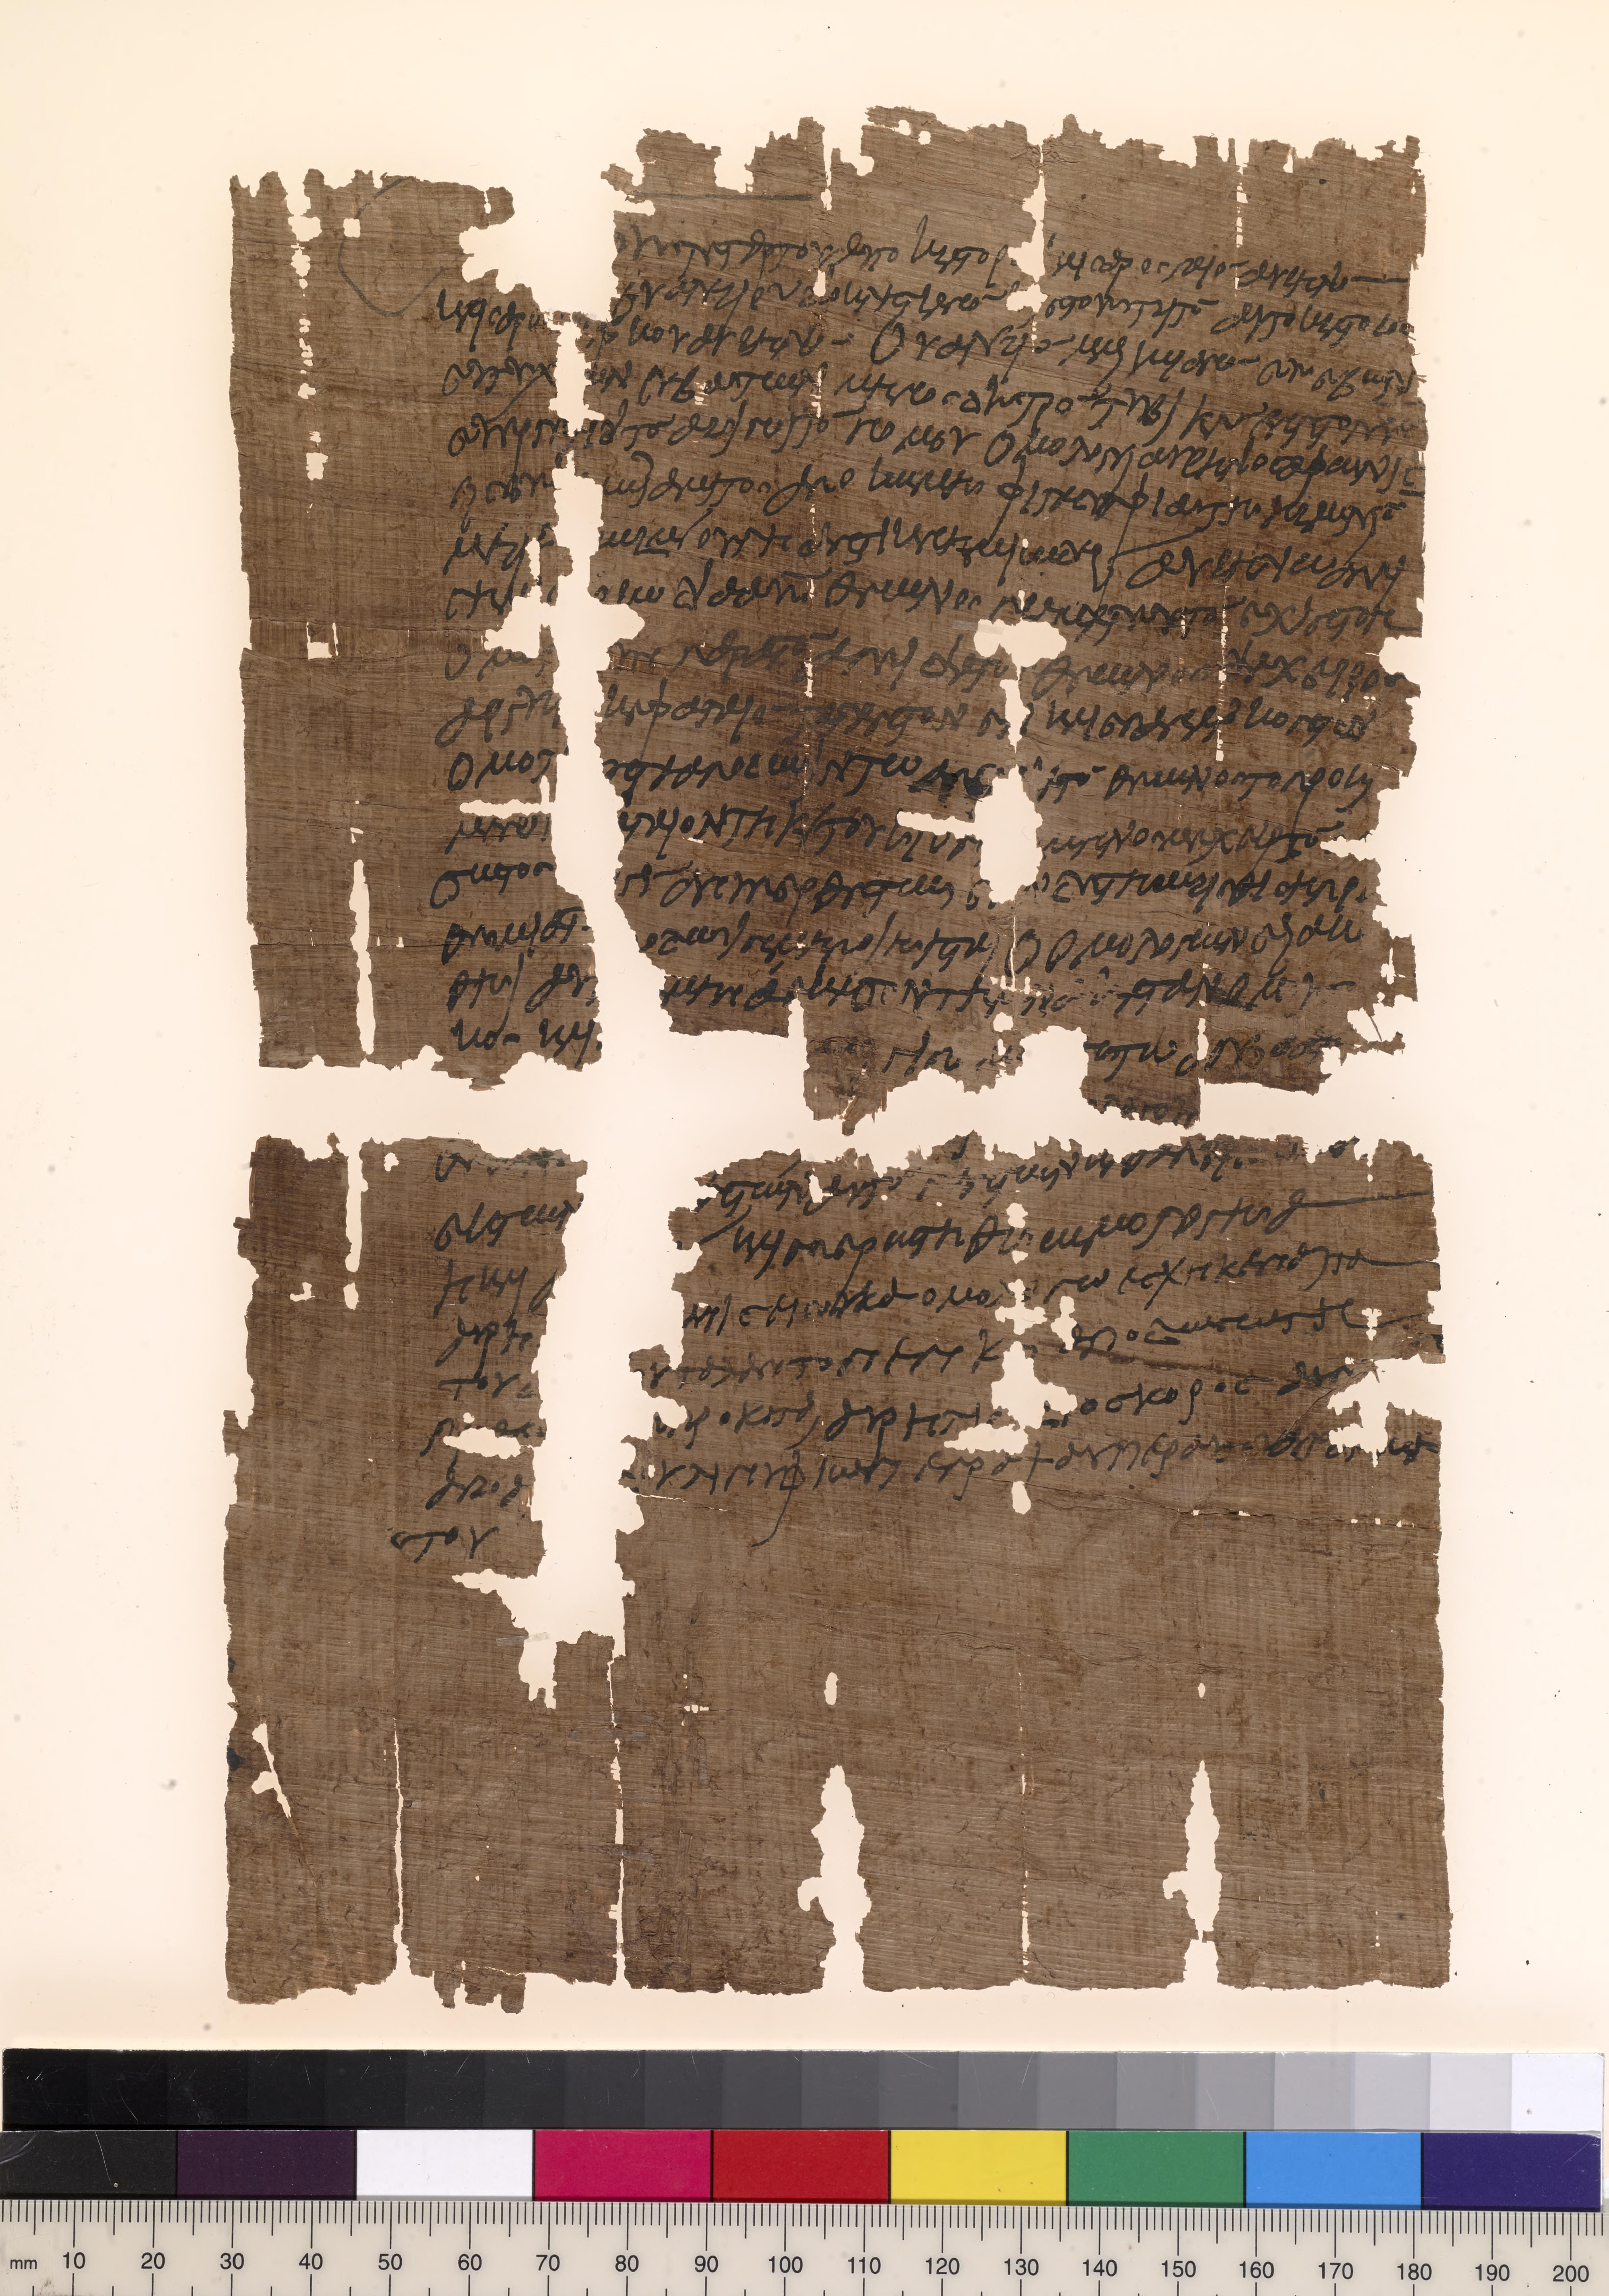
\includegraphics[width=\textwidth]{figures/0_papyri_sample.jpg}
	\caption{A papyri 1398\_1353R torn into several fragments}
	\label{fig:papyri_sample}
\end{figure}
%
\noindent Deep learning algorithms are among the commonly discussed types of algorithms when it comes to supporting papyrologists. Research has shown that the use of deep learning can increase the efficiency of papyrologists. However, even though the results are promising, there are still many unanswered questions that we do not understand. Once a better understanding of the features is obtained, the algorithms can increase the papyrologists's efficiency by a greater chance. 

\section{Contribution}
The general objective of this thesis is to make the work of papyrologists easier and increase their efficiency
by partially automating the reassembling process. To this end, an algorithm is designed to infer a
smaller sub-selection of fragments with a high likelihood of being a potential fit. In the following, this
algorithm is called puzzle-helper. Additionally algorithms have to be in a format that papyrologists can use the algorithm without a computer science background. Also, using deep learning implies that a vast amount of (labeled) data is required. The database from the University of Michigan offers plenty of it. Once the data is downloaded, it must be correctly preprocessed, like removing low contrast images or labeling the data. In particular, this thesis is centered around the following research questions:
\begin{questions}
	\item What papyrus characteristics contribute to the success of papyrus fragment retrieval?
	\item How can papyrologists use fragment retrieval model efficiently?
\end{questions}

\section{Outline}
In \Cref{chap:intro}, the context of this master thesis is explained, and the research questions are defined. Further, it is explained how the thesis is structured. \Cref{chap:Foundation} presents groundbreaking work in all areas that are relevant to this thesis. The objective is to present a quick overview of the state-of-the-art in historical fragment retrieval. \Cref{chap:Datasets} explains the creation of a dataset that can be used for papyri fragment retrieval. The objective is to guide the reader such that it is possible to recreate the dataset quickly. \Cref{chap:theory} serves as a short introduction to the field of deep learning. Further, it will be presented how that technology is used in the field of \ac{cv} for cultural heritage by the example of papyri fragment retrieval. \Cref{chap:methodology} shows how the author of this thesis used \ac{dml} as a methodology for answering the defined research questions. Further it shows how the results have been evaluated with suitable metrics. \Cref{chap:results} summarizes the results. It shows what was achieved while conducting the experiments and evaluating the results according to the defined metrics. \Cref{chap:application} shows how the results can be efficiently presented to an audience of papyrologists without \ac{cv} capabilities. \Cref{chap:discussion} revisits the research questions and summarizes the key findings. Furthermore, the results are interpreted and discussed to align with the defined research questions. Finally, the author of this thesis presents optional future work and finalizes his work with a summary. 